\section{Условие задачи}

Группа из 8 человек, длительность не более 4 месяцев, бюджет не более 620 тысяч рублей.

\section{Задание 1}

\begin{figure}[H]
    \centering
    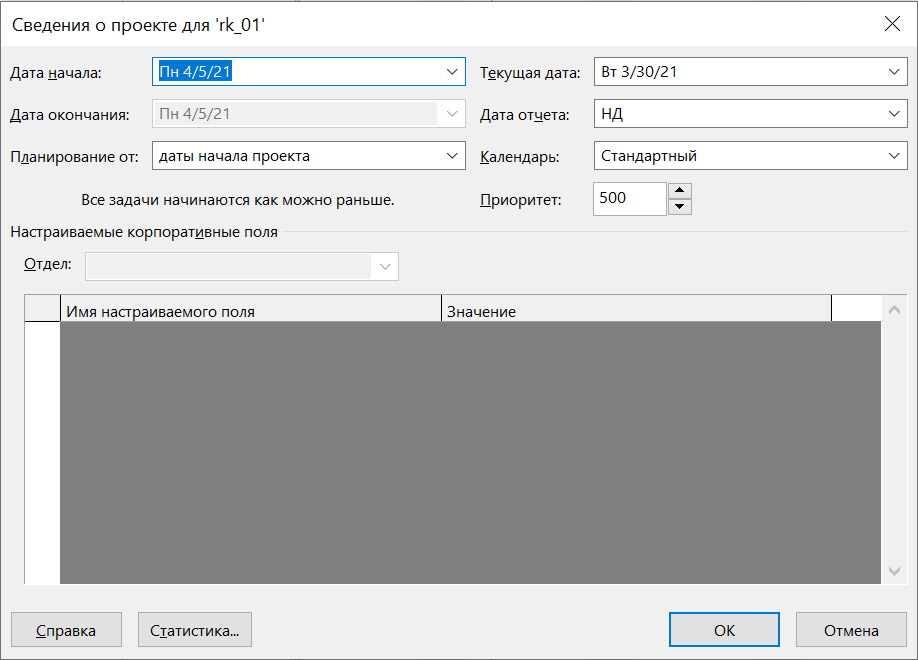
\includegraphics[width=0.7\textwidth]{img/content/task_01_1.png}
    \caption{Установка даты начала проекта}
    \label{fig:task_01_1}
\end{figure}

\begin{figure}[H]
    \centering
    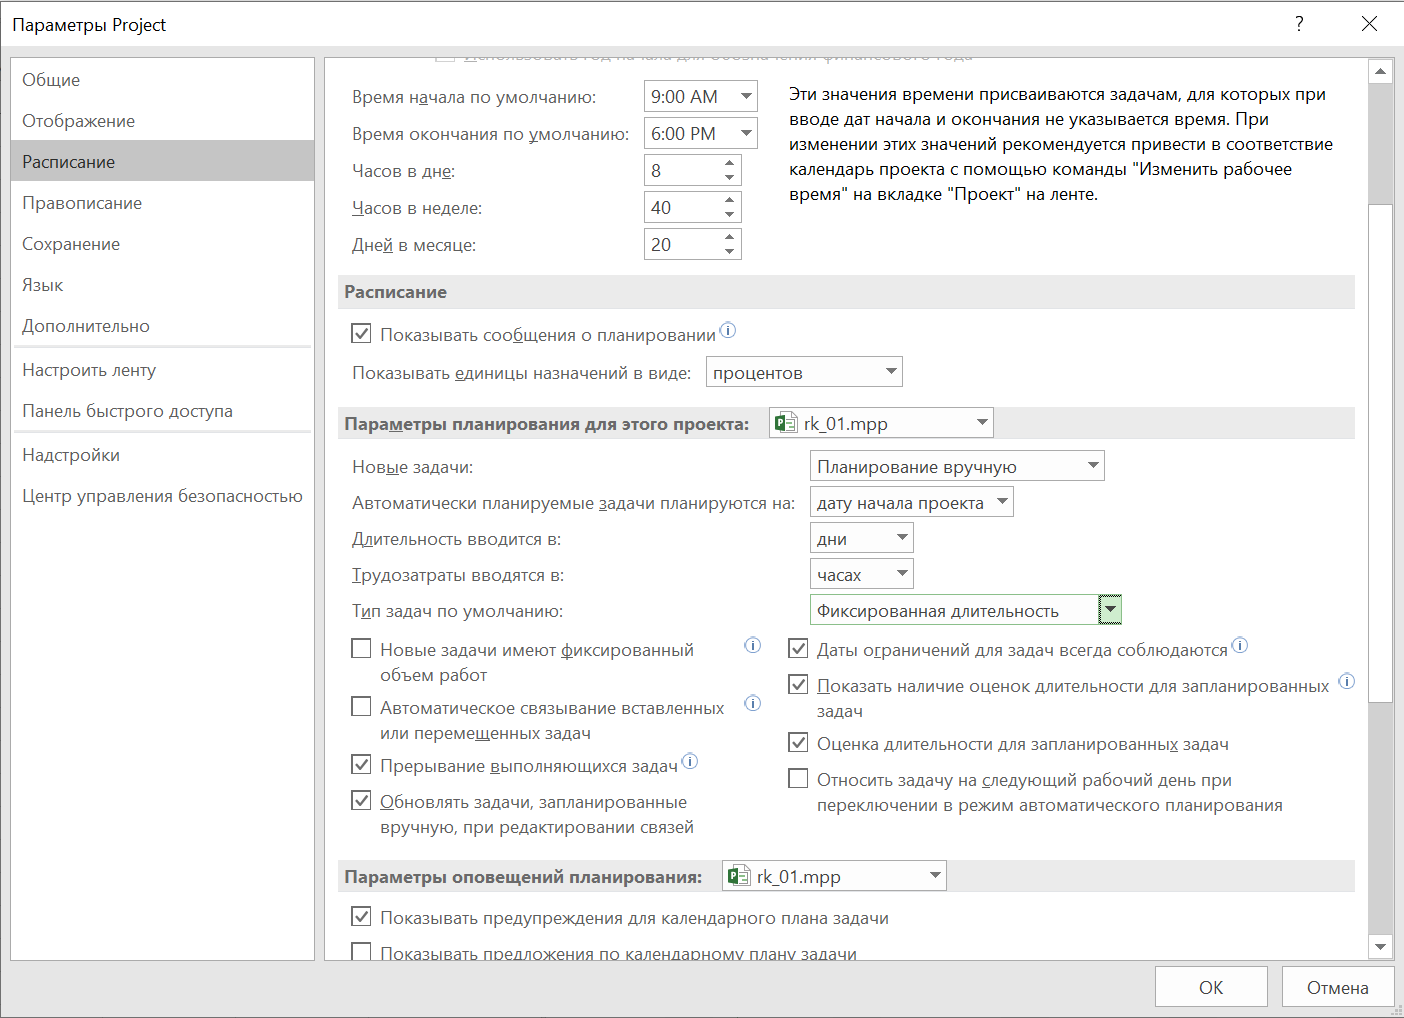
\includegraphics[width=0.7\textwidth]{img/content/task_01_2.png}
    \caption{Настройка проекта}
    \label{fig:task_01_2}
\end{figure}

\begin{figure}[H]
    \centering
    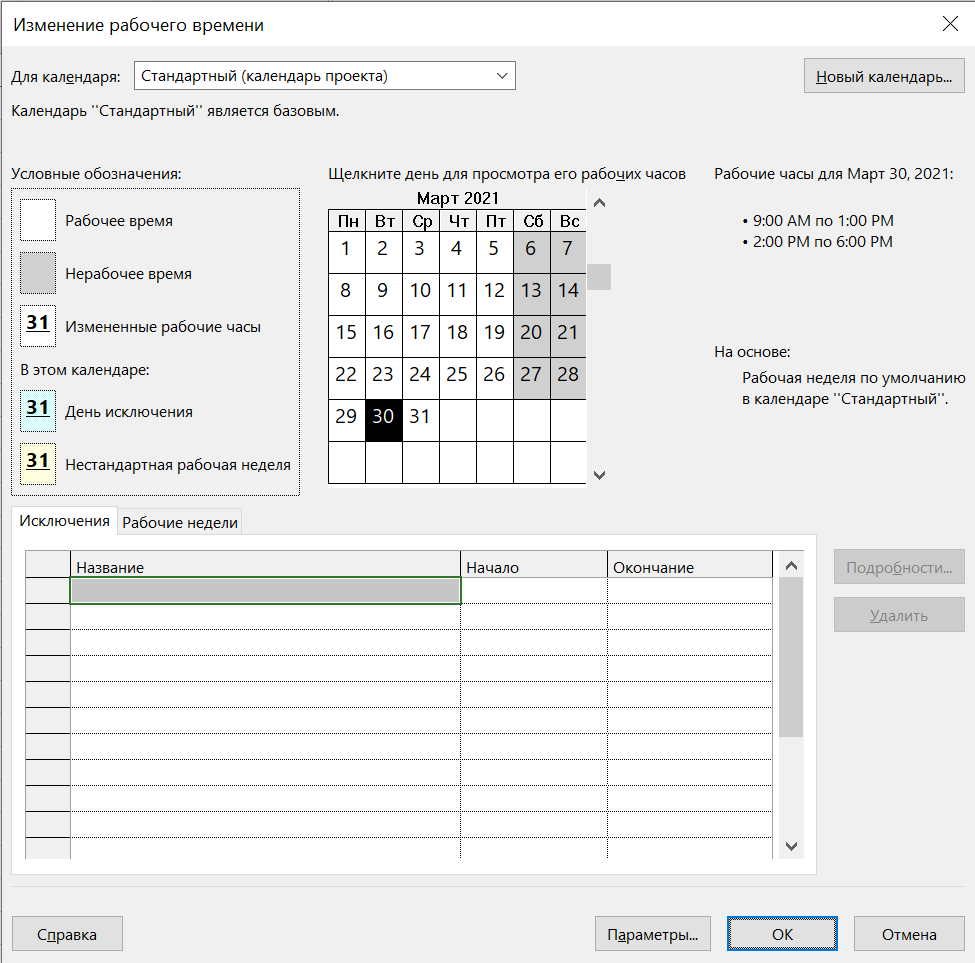
\includegraphics[width=0.6\textwidth]{img/content/task_01_3.png}
    \caption{Установка стандартного календаря}
    \label{fig:task_01_3}
\end{figure}

\begin{figure}[H]
    \centering
    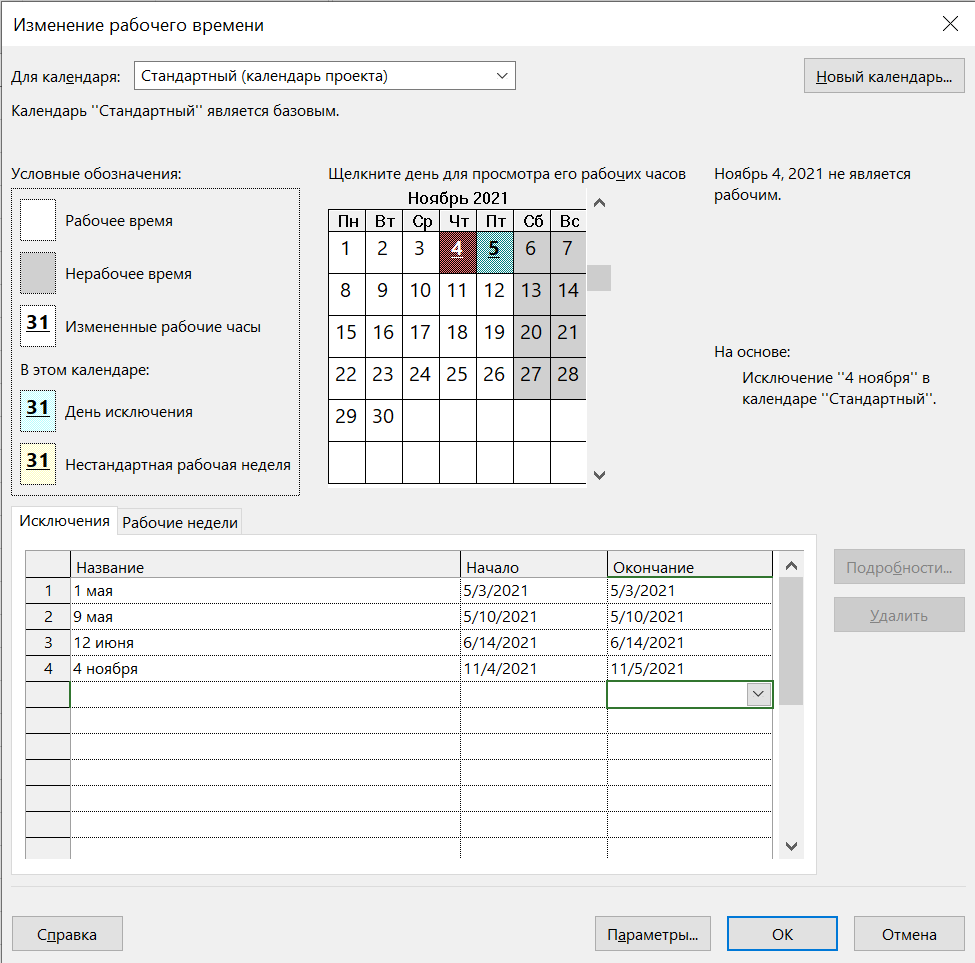
\includegraphics[width=0.6\textwidth]{img/content/task_01_4.png}
    \caption{Учет празников}
    \label{fig:task_01_4}
\end{figure}

\section{Задание 2}

\begin{figure}[H]
    \centering
    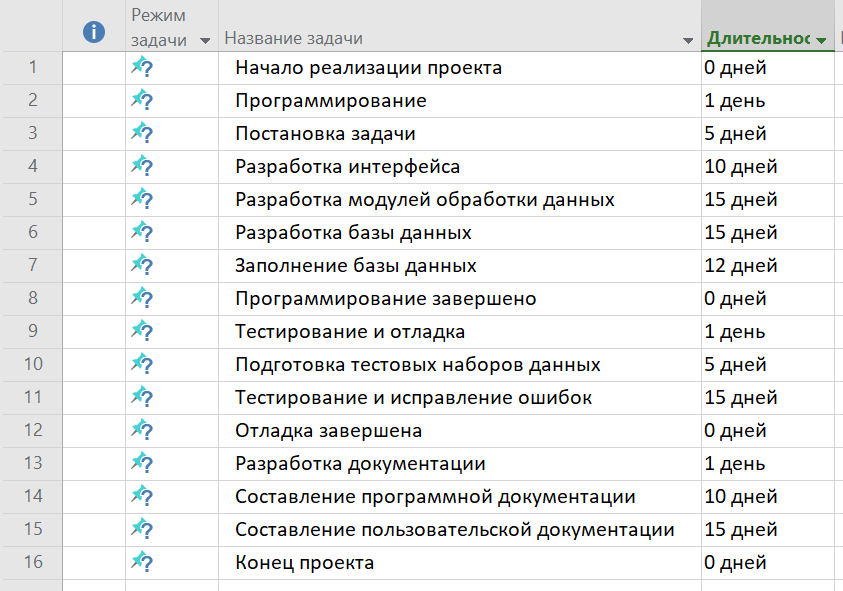
\includegraphics[width=0.8\textwidth]{img/content/task_02.png}
    \caption{Список задач}
    \label{fig:task_02}
\end{figure}

\section{Задание 3}

\begin{figure}[H]
    \centering
    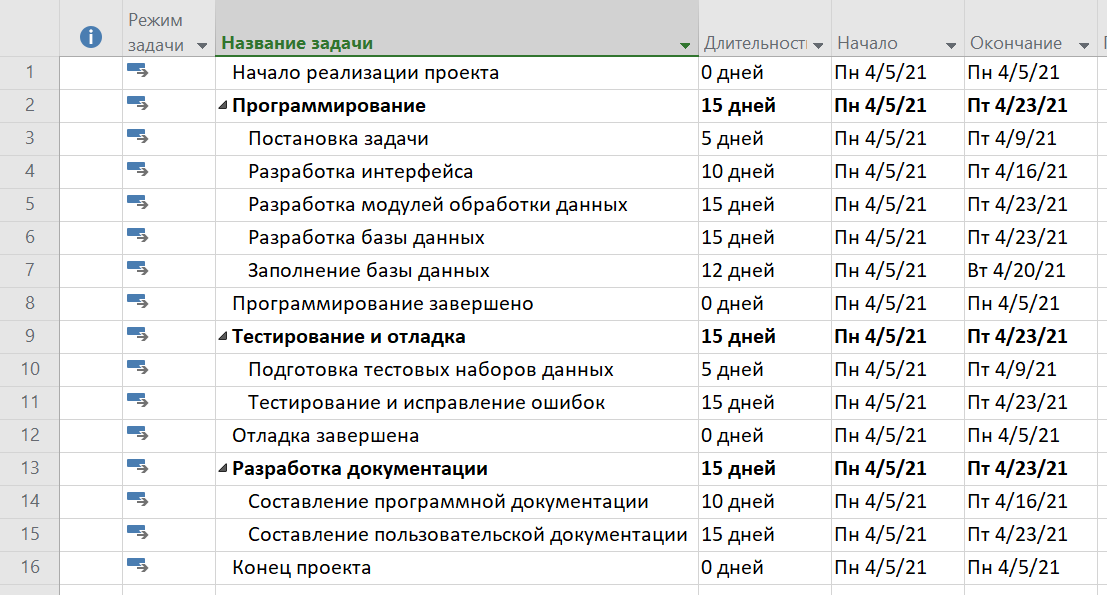
\includegraphics[width=0.8\textwidth]{img/content/task_03.png}
    \caption{Группировка задач}
    \label{fig:task_03}
\end{figure}

\section{Задание 4}

\begin{figure}[H]
    \centering
    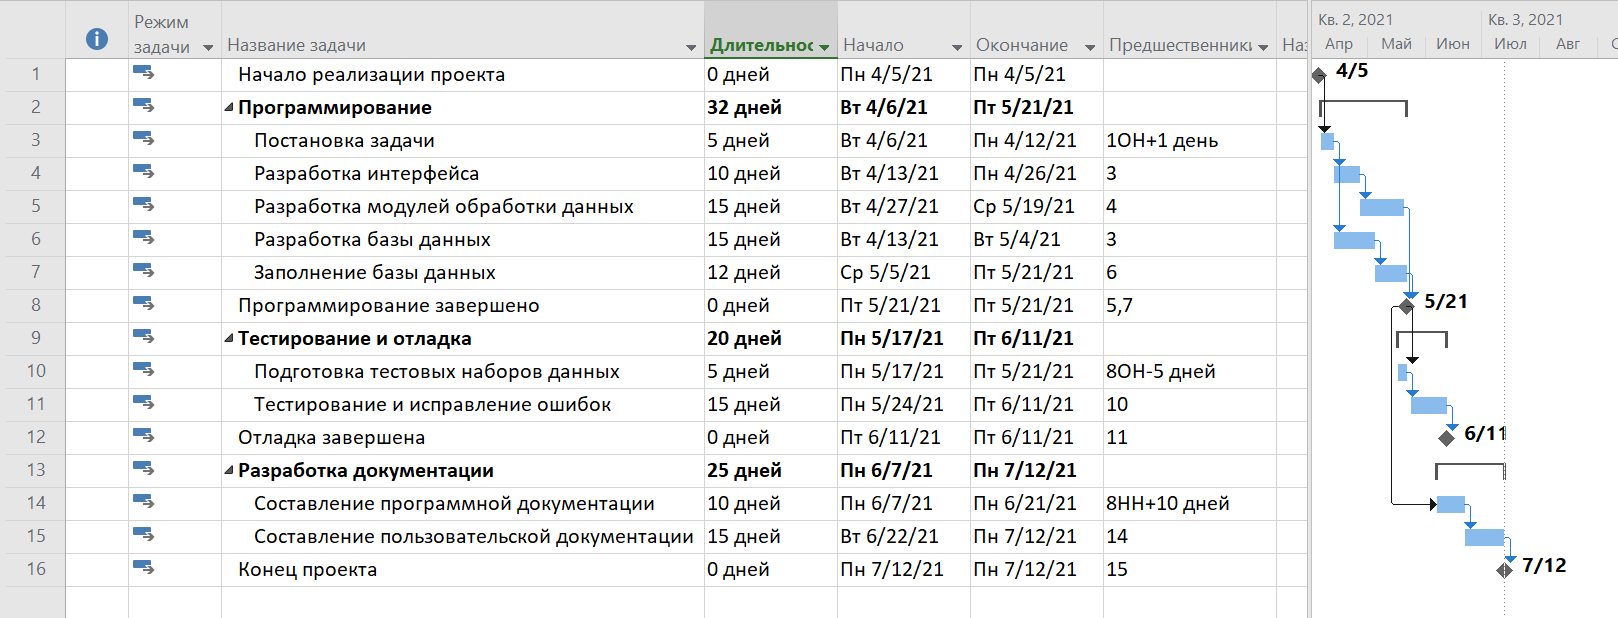
\includegraphics[width=0.8\textwidth]{img/content/task_04.png}
    \caption{Установление связей между задачами}
    \label{fig:task_04}
\end{figure}

\section{Задание 5}

\begin{figure}[H]
    \centering
    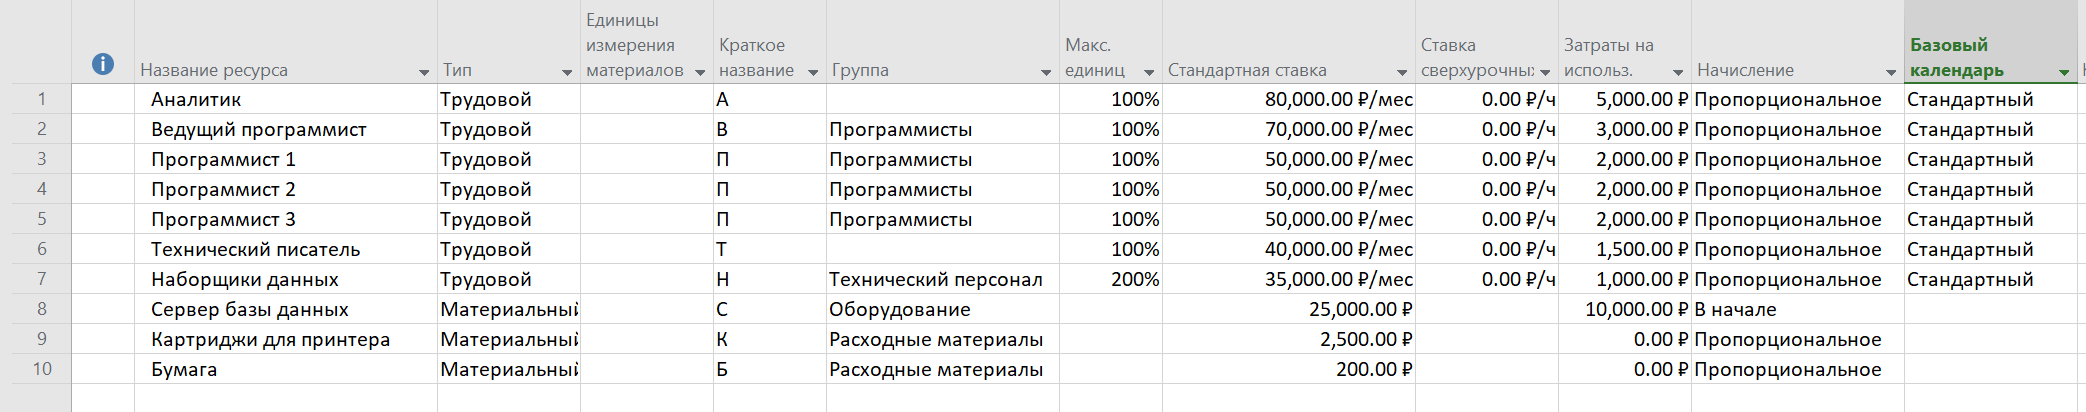
\includegraphics[width=0.8\textwidth]{img/content/task_05_1.png}
    \caption{Создание списка ресурсов}
    \label{fig:task_05_1}
\end{figure}

\begin{figure}[H]
    \centering
    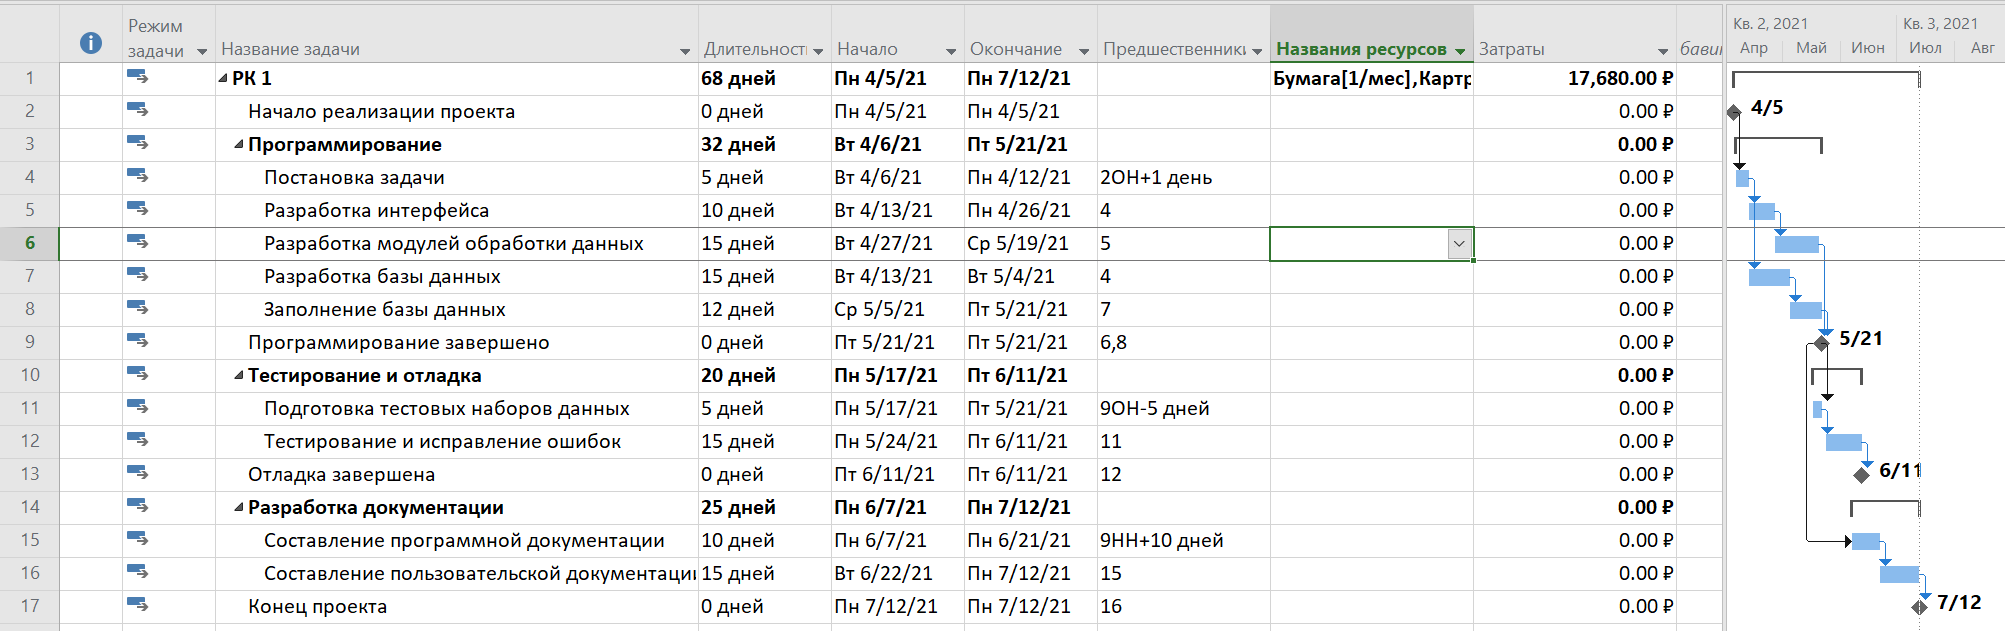
\includegraphics[width=0.8\textwidth]{img/content/task_05_2.png}
    \caption{Назначение расхода бумаги и картриджей на суммарную задачу}
    \label{fig:task_05_2}
\end{figure}

\section{Задание 6}

\begin{figure}[H]
    \centering
    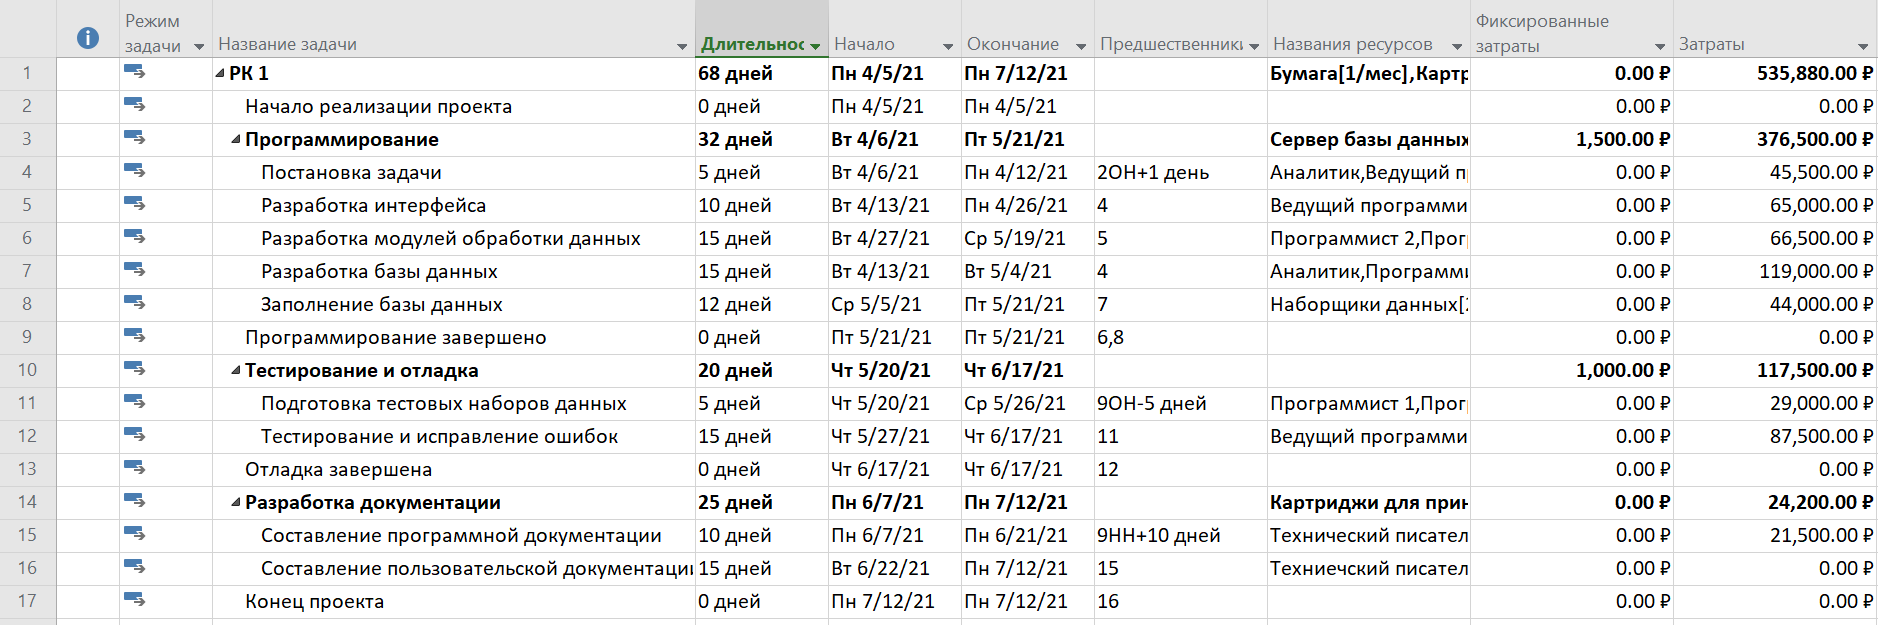
\includegraphics[width=0.8\textwidth]{img/content/task_06.png}
    \caption{Назначение ресурсов и затрат для задач}
    \label{fig:}
\end{figure}

\section{Задание 7}

Перегрузки ресурсов после распределения их по задачам не произошло.

В итоге получаем, что задача укладывается в рамки. Окончание задачи планируется 12 июля, а бюджет 535 880 рублей.

\section{Задание 8}

\begin{figure}[H]
    \centering
    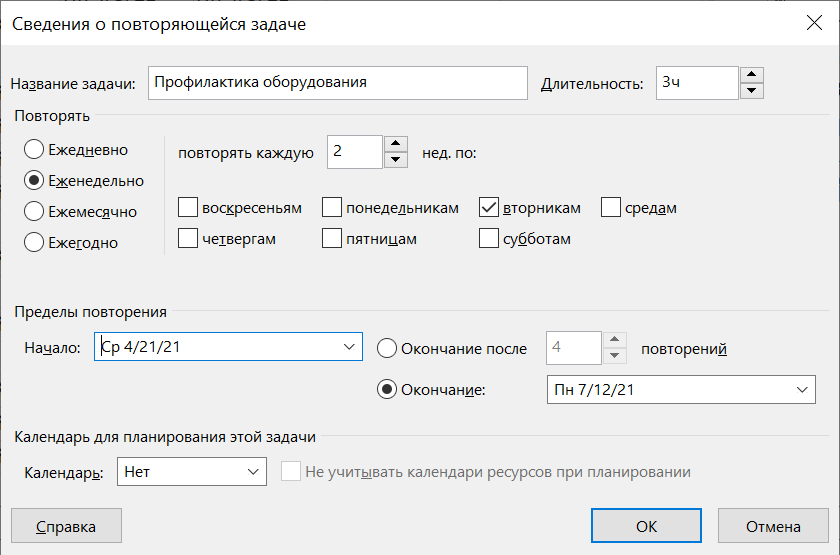
\includegraphics[width=0.8\textwidth]{img/content/task_08_1.png}
    \caption{Создание повторяющейся задачи}
    \label{fig:task_08_1}
\end{figure}

Необходимо учесть в затраты проекта договор с компанией, предусматривающий выезд специалиста для профилактики. Стоимость одного выезда 3000 рублей. Создадим новый ресурс <<Специалист по профилактике>> и заведем для него стаку 0 рублей, а затраты на использование 3000 рублей.

\begin{figure}[H]
    \centering
    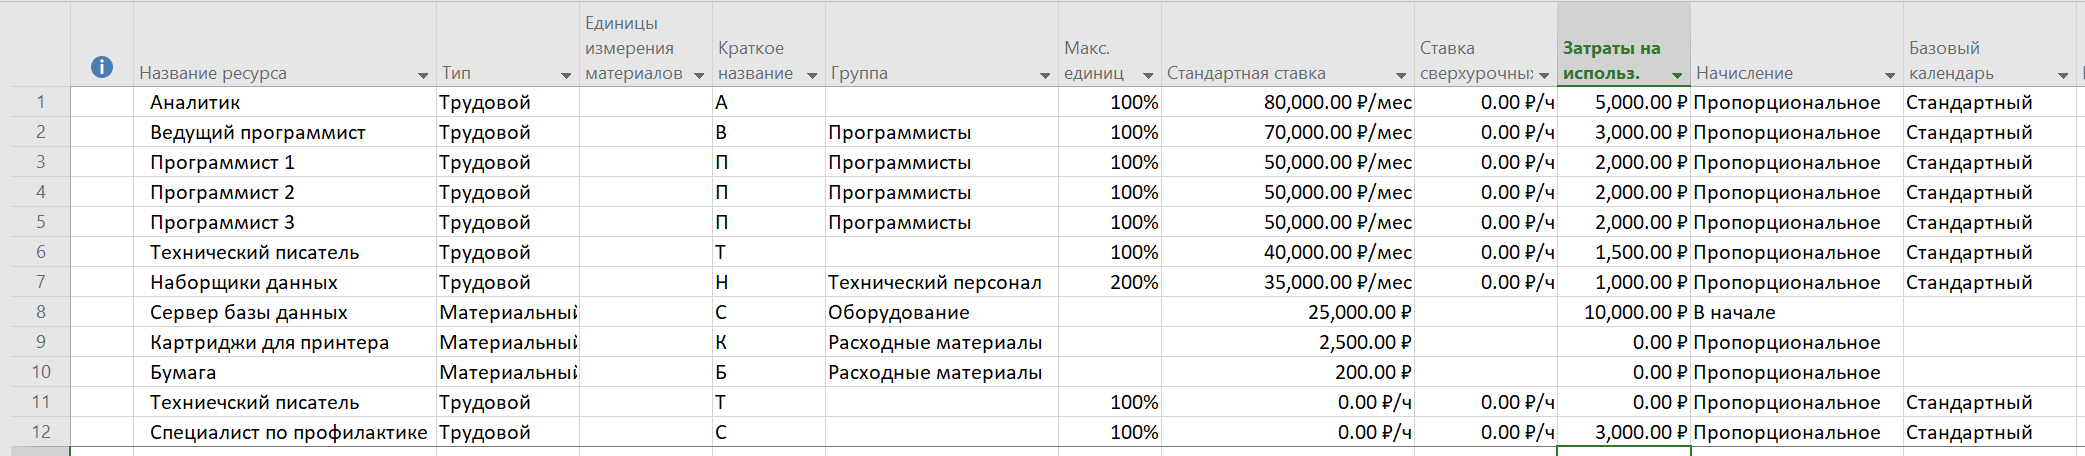
\includegraphics[width=0.8\textwidth]{img/content/task_08_2_1.png}
    \caption{Создание нового ресурса}
    \label{fig:task_08_2_1}
\end{figure}

\begin{figure}[H]
    \centering
    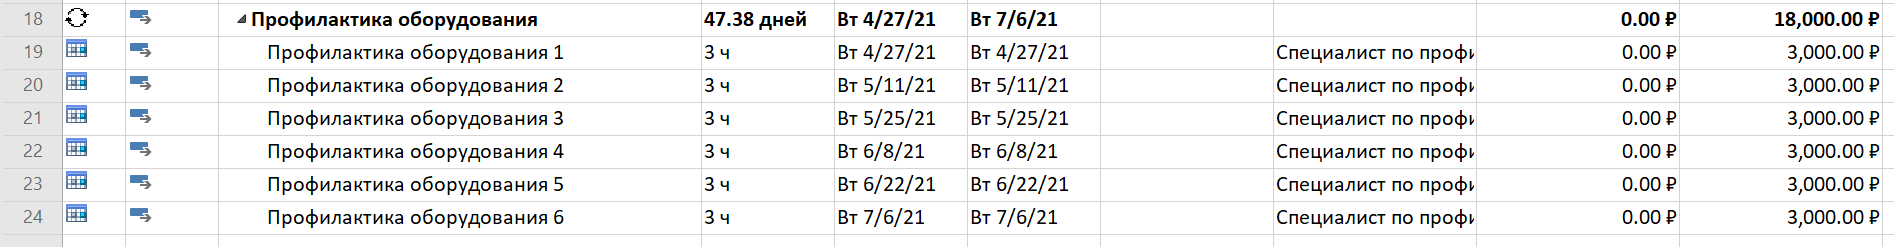
\includegraphics[width=0.8\textwidth]{img/content/task_08_2_2.png}
    \caption{Распределение нового ресурса по задачам}
    \label{fig:task_08_2_2}
\end{figure}

Необходимо учесть, что во время профилактики никакие задачи не могут выполняться. Создадим исключения для всех дней, в которые проводится профилактика и снизим рабочий день на три часа.

\begin{figure}[H]
    \centering
    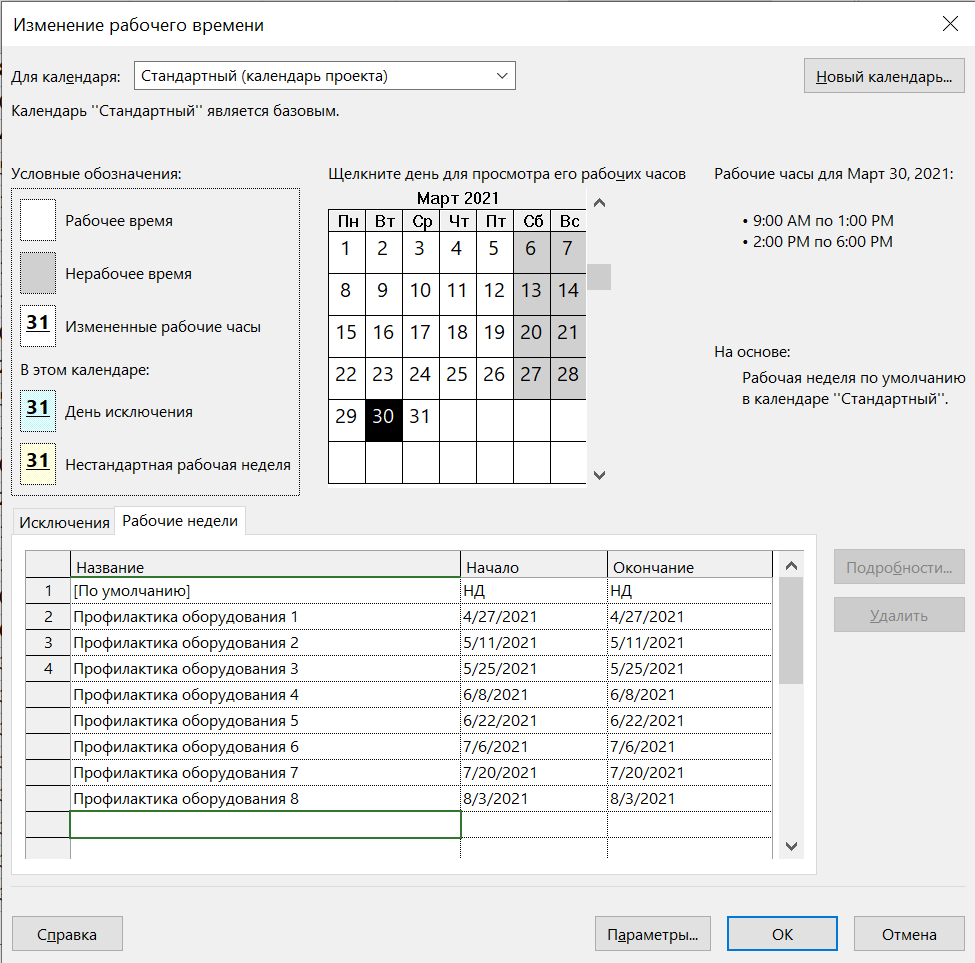
\includegraphics[width=0.8\textwidth]{img/content/task_08_3_1.png}
    \caption{Создание исключений для всех профилактик}
    \label{fig:task_08_3_1}
\end{figure}

\begin{figure}[H]
    \centering
    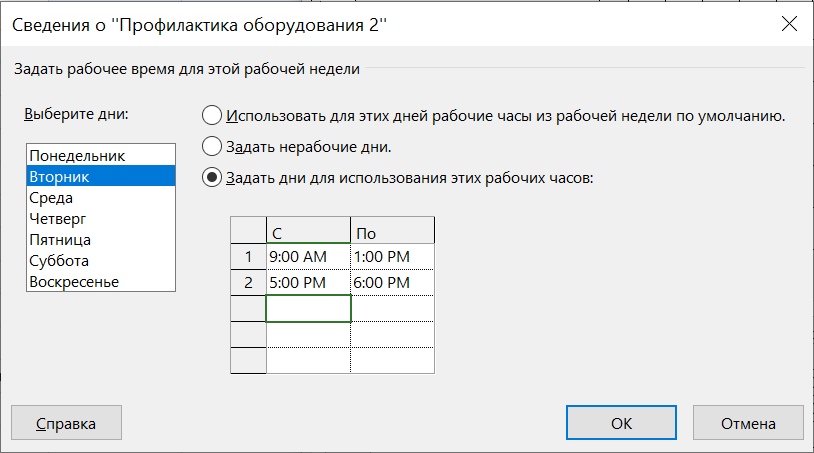
\includegraphics[width=0.8\textwidth]{img/content/task_08_3_2.png}
    \caption{Снижение рабочего дня на три часа для дней с профилактикой}
    \label{fig:task_08_3_2}
\end{figure}

\begin{figure}[H]
    \centering
    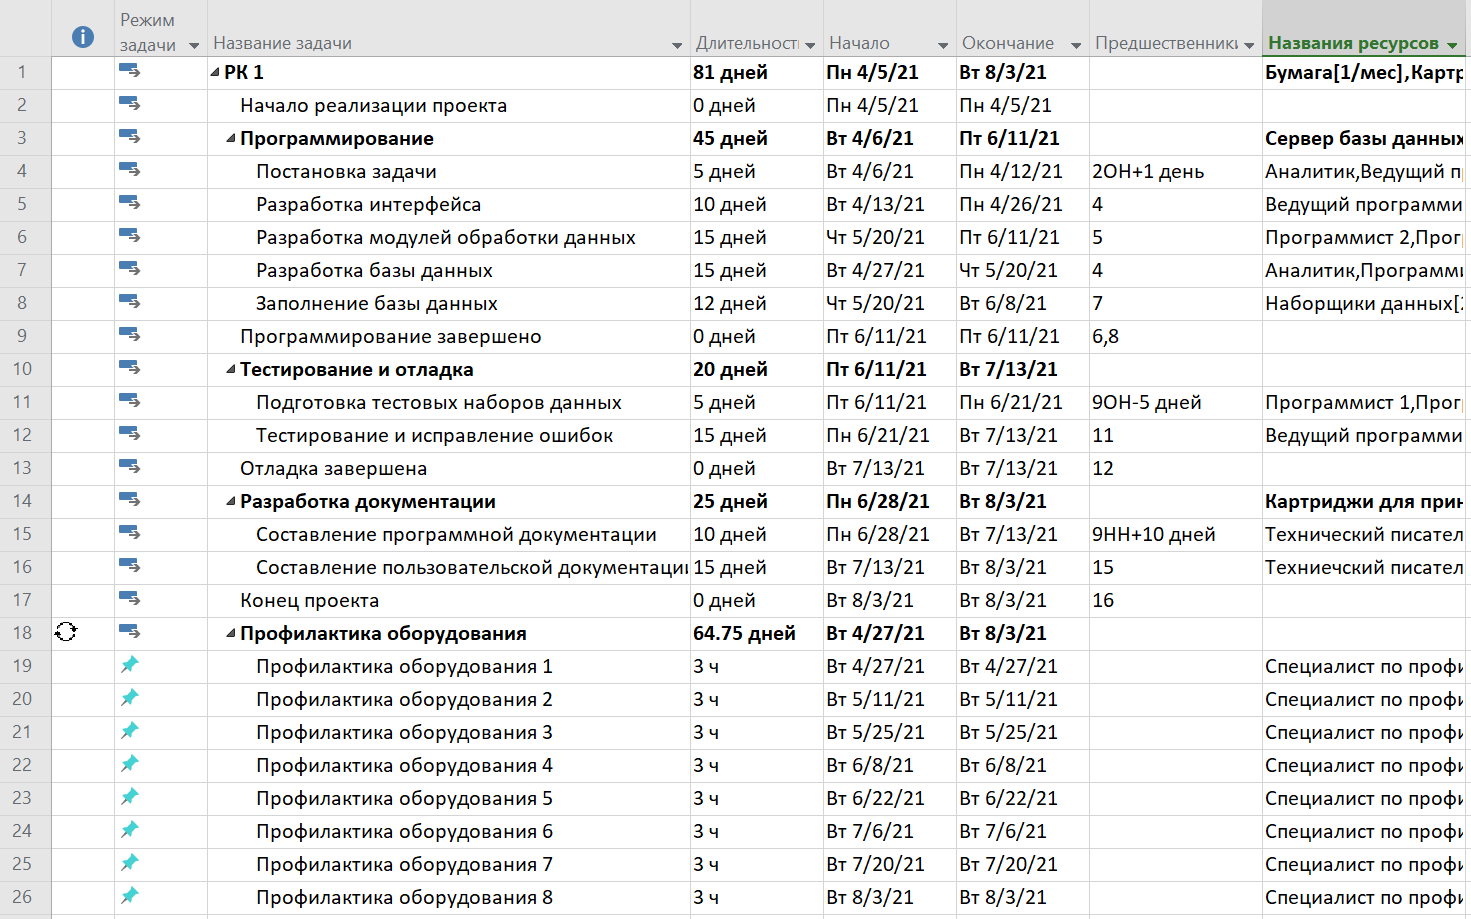
\includegraphics[width=0.8\textwidth]{img/content/task_08_finish.png}
    \caption{Результат добавления профилактики}
    \label{fig:task_08_finish}
\end{figure}

В результате добавления профилактики раз в две недели сроки проекта сдвинулись до 3 августа (на 22 дня позже).

\section{Задание 9}

Для оптимизации проекта были назначены все программисты, кроме ведущего на все задачи, связанные с программированием. В результате проведенной оптимизаци сроки сдвинулись до 19 июля (на 15 дней раньше).

\begin{figure}[H]
    \centering
    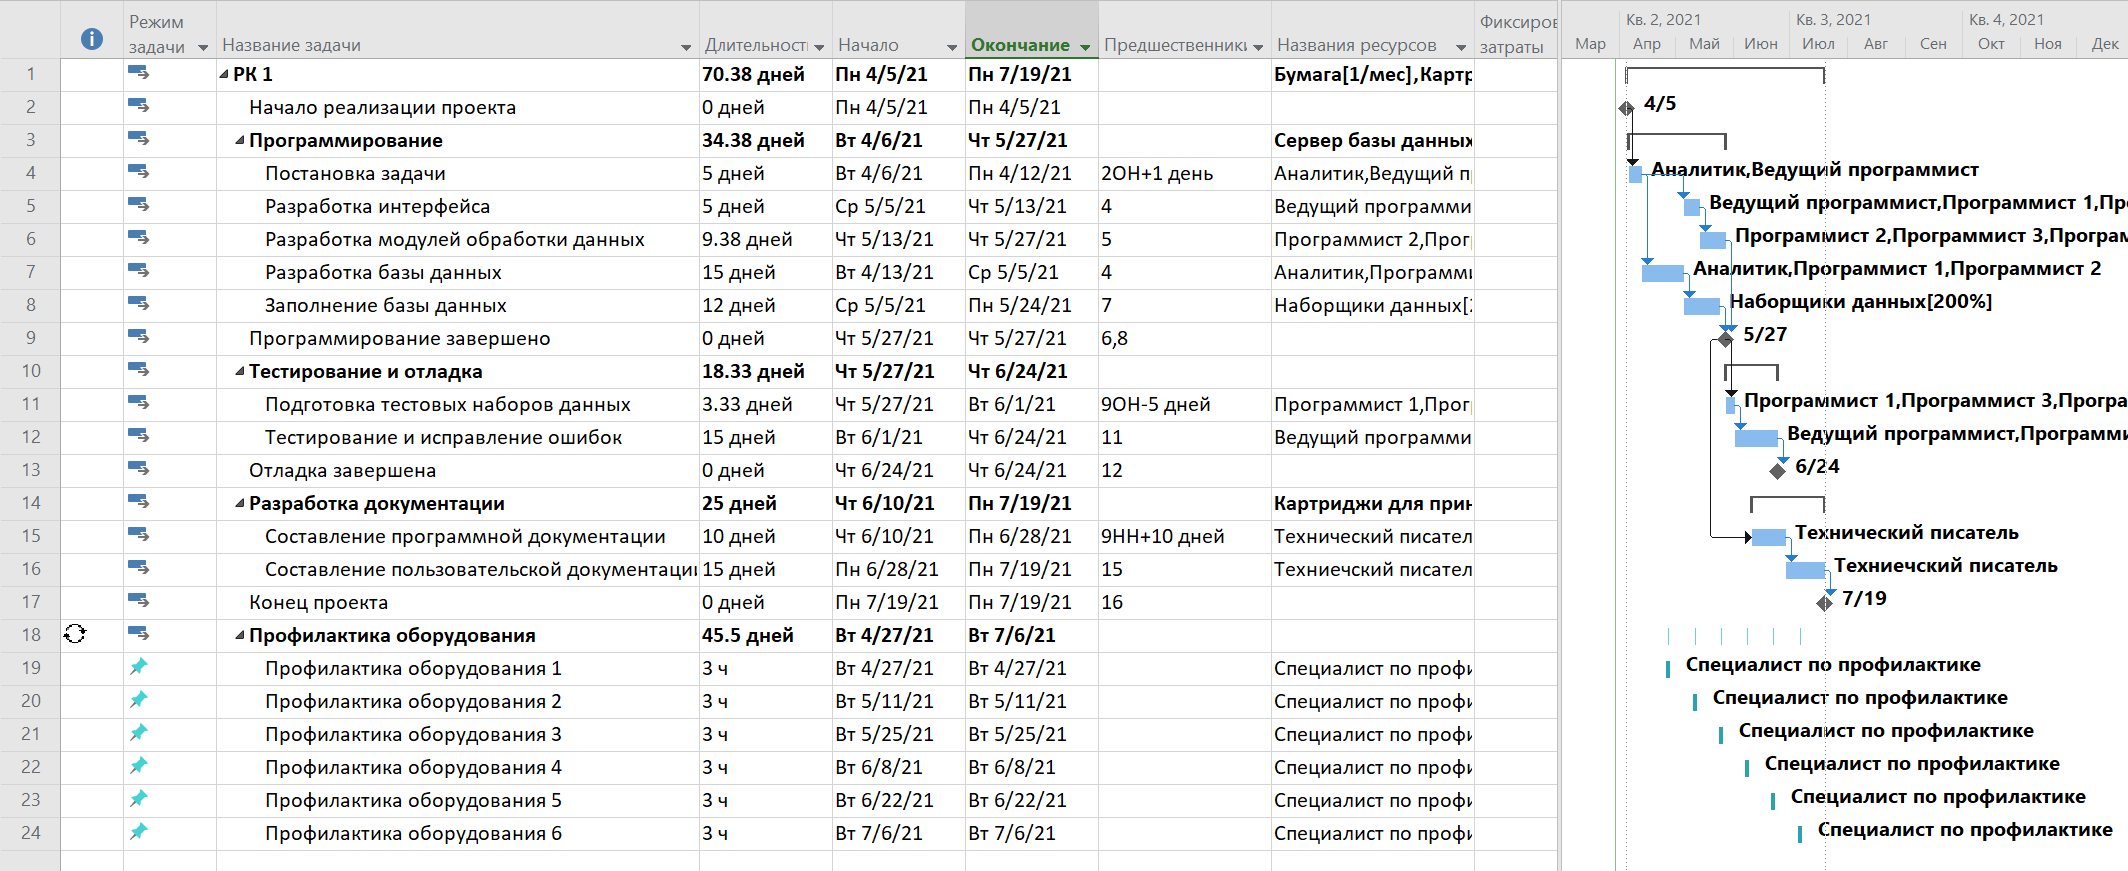
\includegraphics[width=0.8\textwidth]{img/content/task_09_1.png}
    \caption{Результат проведенной оптимизации}
    \label{fig:task_09_1}
\end{figure}

\begin{figure}[H]
    \centering
    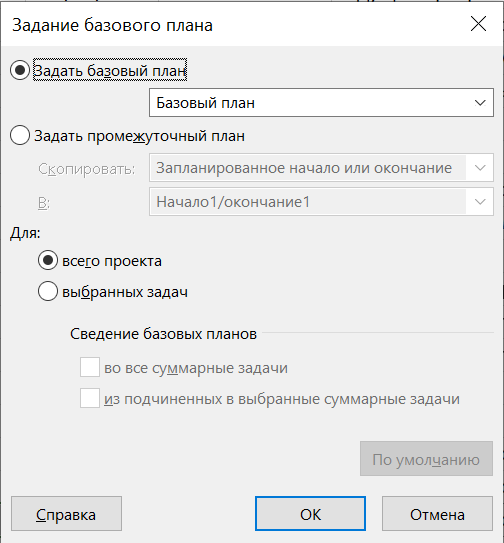
\includegraphics[width=0.8\textwidth]{img/content/task_09_2.png}
    \caption{Задание базового плана}
    \label{fig:task_09_2}
\end{figure}

\section{Задание 10}

Дата отчета -- 1 июля 2021.

Фактические данные:

\begin{itemize}
    \item Наборщик данных сломал себе палец во время кропотливой работы (ушел на больничный с 7 мая)
    \item Ведущий программист получил повышение зарплаты на 10\% с 1 мая
    \item Задача <<Разработка модулей обработки данных>> потребовала в два раза больше времени
\end{itemize}

\begin{figure}[H]
    \centering
    
\includegraphics[width=0.8\textwidth]{img/content/task_10_1_1.png}
    \caption{Уменьшение доступных ресурсов наборщиков до 1 человека}
    \label{fig:task_10_1_1}
\end{figure}

\begin{figure}[H]
    \centering
    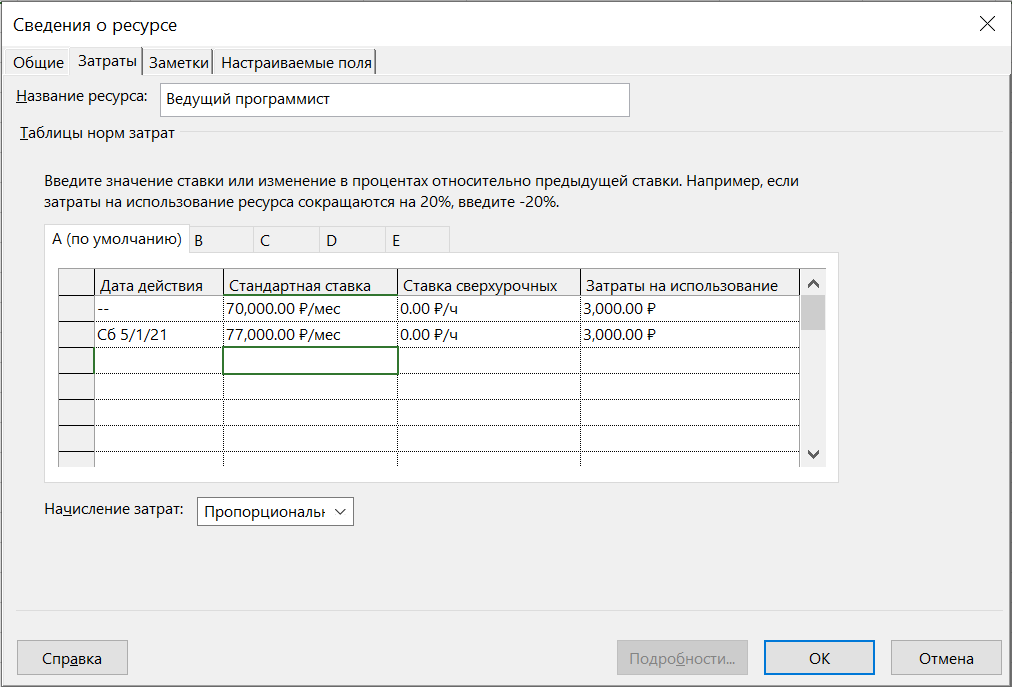
\includegraphics[width=0.8\textwidth]{img/content/task_10_1_2.png}
    \caption{Повышение зарплаты ведущему программисту}
    \label{fig:task_10_1_2}
\end{figure}

\begin{figure}[H]
    \centering
    
\includegraphics[width=0.8\textwidth]{img/content/task_10_1_3.png}
    \caption{Увеличение выполнения задачи в два раза дольше}
    \label{fig:task_10_1_3}
\end{figure}

\begin{figure}[H]
    \centering
    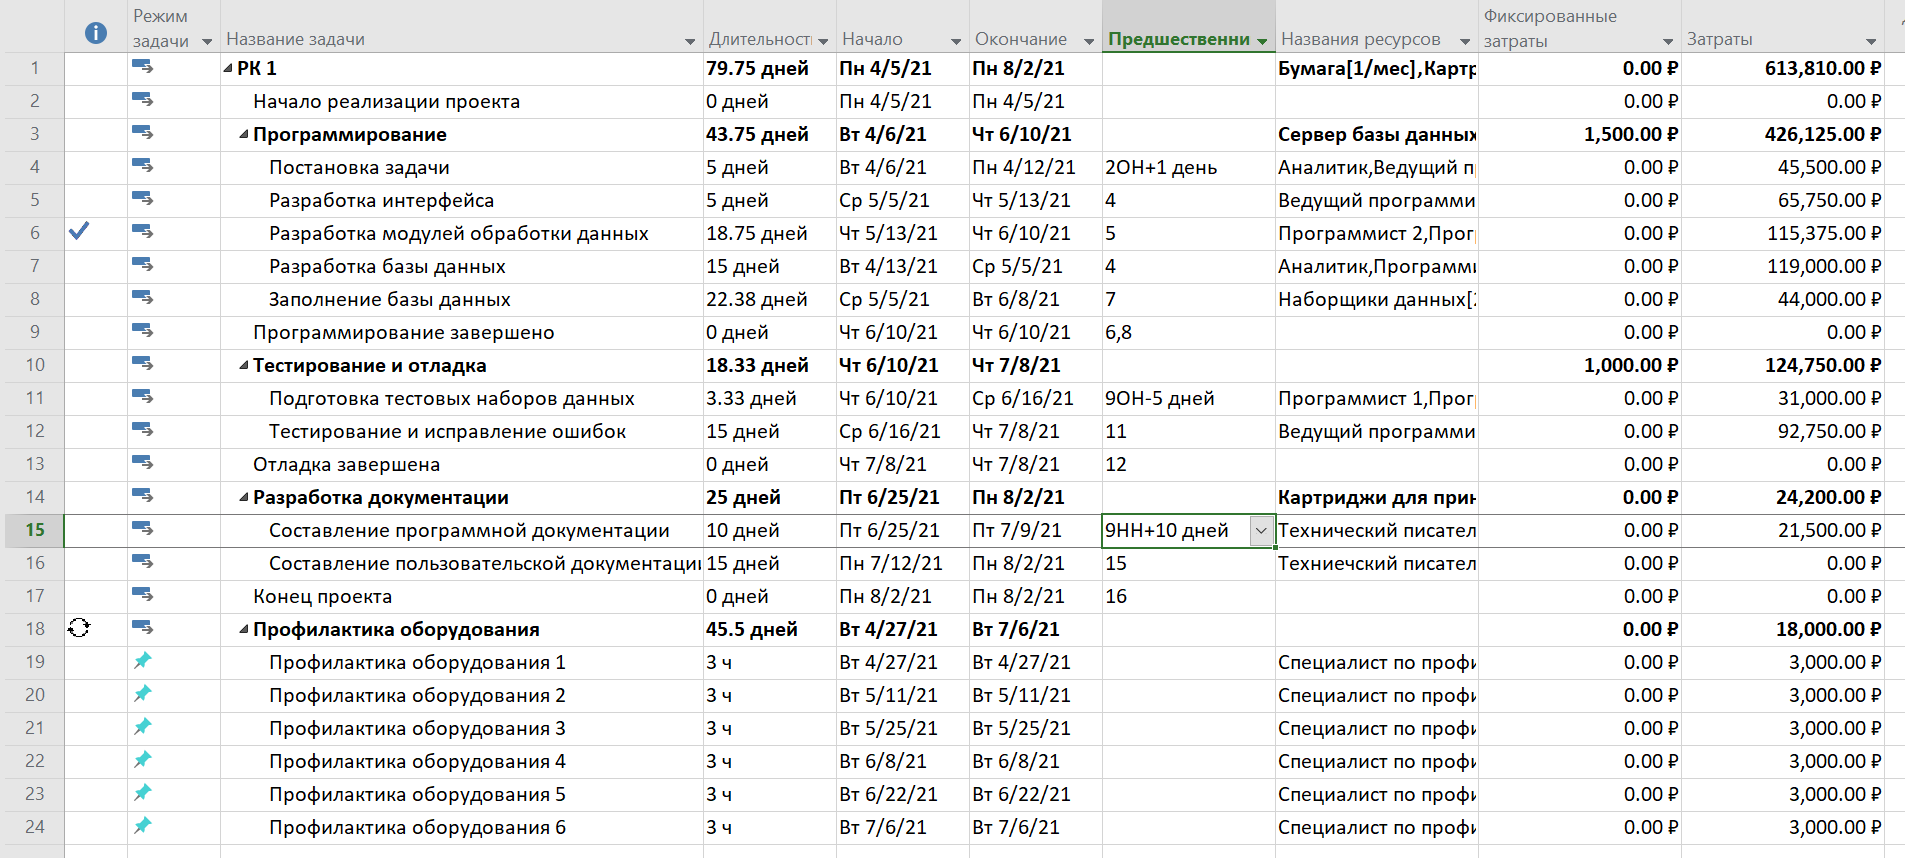
\includegraphics[width=0.8\textwidth]{img/content/task_10_1_finish.png}
    \caption{Результат добавления фактических данных}
    \label{fig:task_10_1_finish}
\end{figure}

В результате внесения фактических данных сроки проекта сдвинулись до 2 августа, а бюджет увеличился до 613 810 рублей, что укладывается в установленные рамки.

\begin{figure}[H]
    \centering
    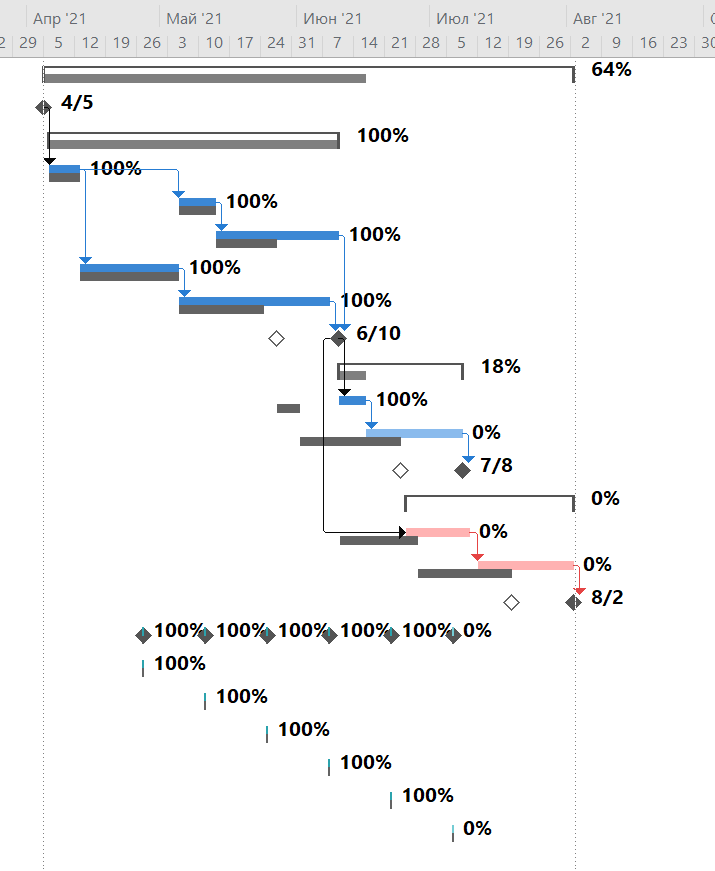
\includegraphics[width=0.8\textwidth]{img/content/task_10_2.png}
    \caption{Отклонения от базового плана}
    \label{fig:task_10_2}
\end{figure}

По отклонениям от базового плана видно, что все задачи выполнились позже, чем планировалось.

\begin{figure}[H]
    \centering
    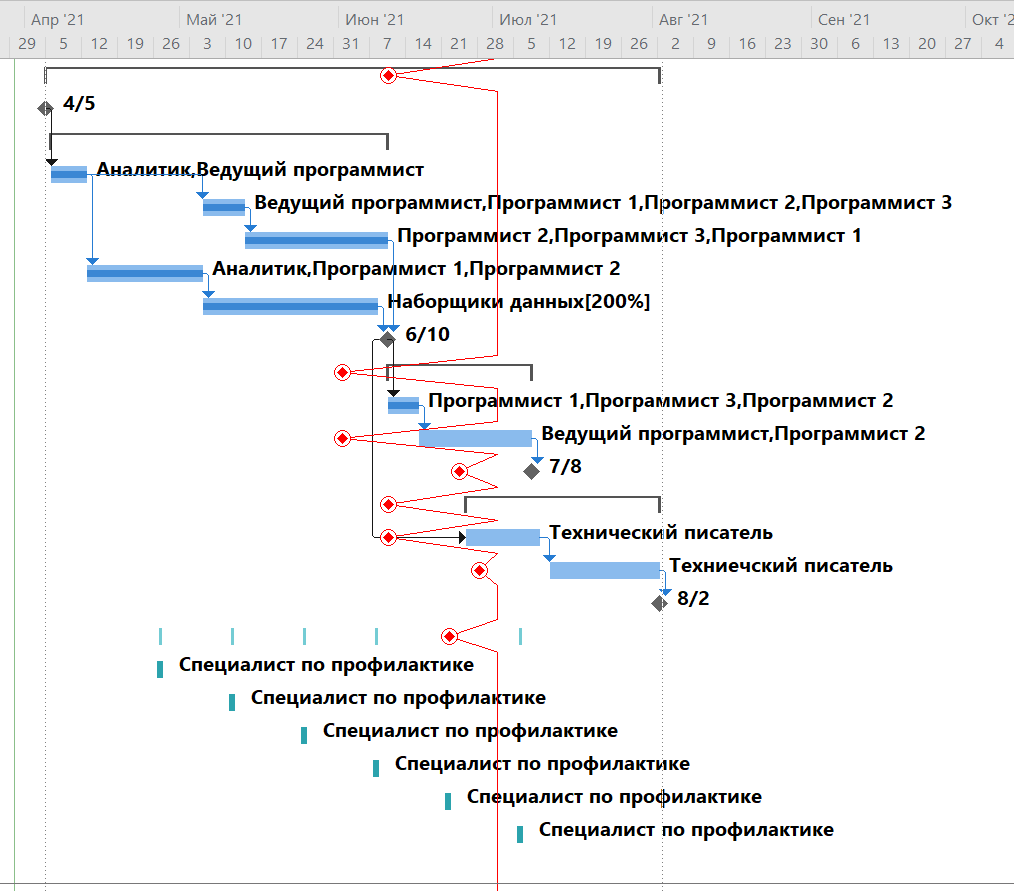
\includegraphics[width=0.8\textwidth]{img/content/task_10_3.png}
    \caption{Линия прогресса}
    \label{fig:task_10_3}
\end{figure}

По линии прогресса видно, что мы отстаем от базового плана.

\begin{figure}[H]
    \centering
    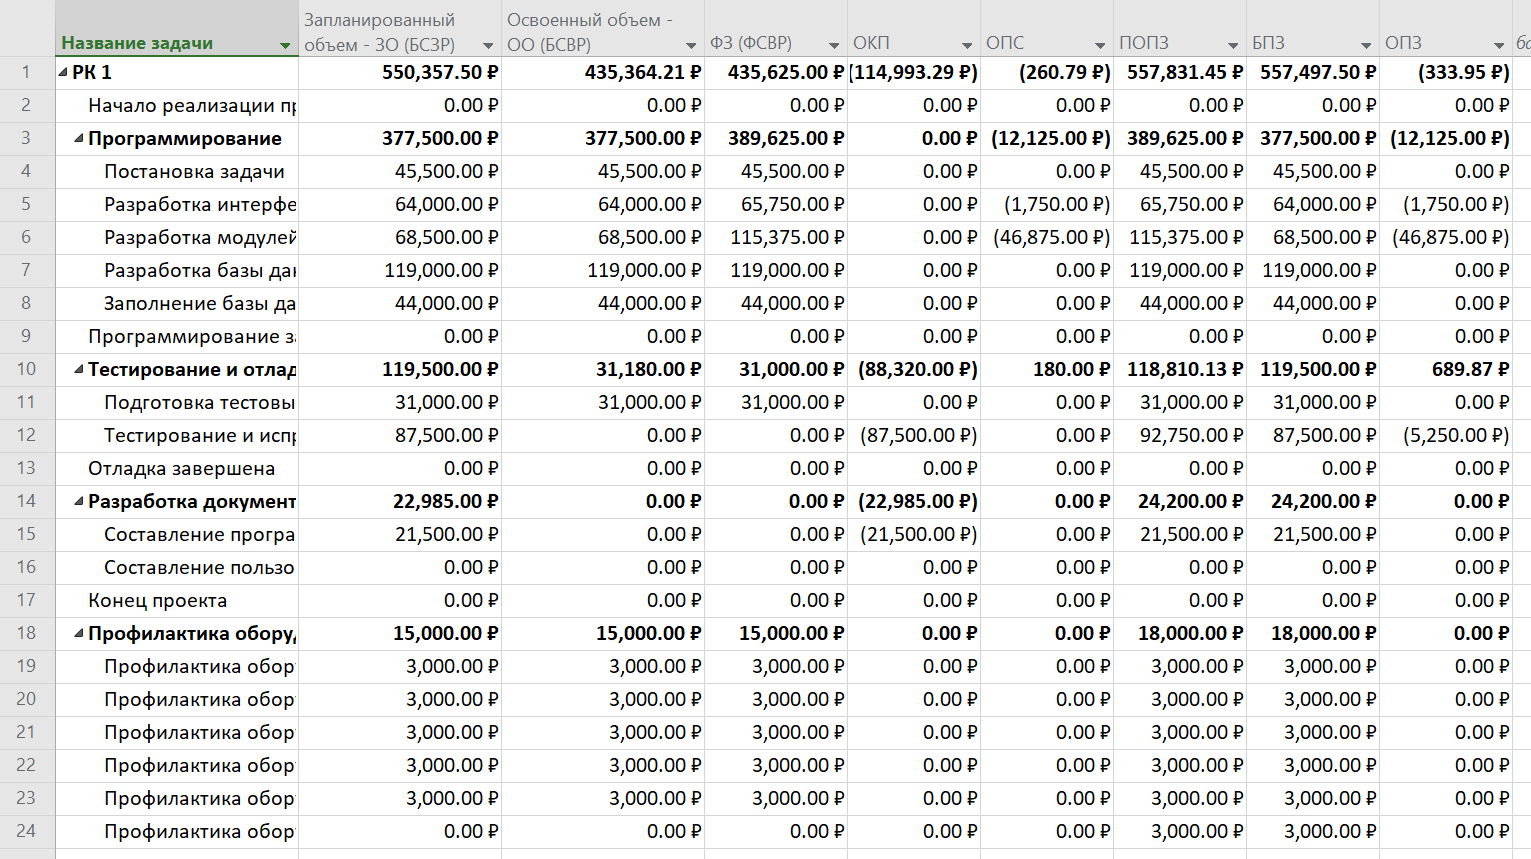
\includegraphics[width=0.8\textwidth]{img/content/task_10_4.png}
    \caption{Освоенный объем проекта}
    \label{fig:task_10_4}
\end{figure}

ЗО = 550 357.50 рублей

БСВР = 435 364.21 рублей

ФЗ = 435 625 рублей

ОКП = 114 993.29 рублей

ПОПЗ = 557 831.45 рублей

БПЗ = 557497.50 рублей

По таблице видно, что по бюджету все укладывается.
